\chapter{Génétique du développement et évolution des formes}\label{ch:b3:developmental-genetics}

L'œuf d'une mouche du vinaigre fait un demi-millimètre de long et, dans
les trois heures qui suivent la fécondation, avant qu'une seule membrane
cellulaire se soit formée entre ses six mille noyaux, il décide quelle
extrémité sera la tête, laquelle la queue, où se placera chacun de
quatorze segments, et lesquels porteront pattes, ailes ou antennes. Il
le fait avec quelques dizaines de gènes, allumés selon une hiérarchie de
bandes de plus en plus fines, chaque bande lue dans les concentrations
des produits des bandes précédentes. En 1980 deux jeunes scientifiques
de Heidelberg criblèrent des milliers de mouches mutantes à la recherche
de larves aux parties manquantes ou doublées, et trouvèrent toute la
hiérarchie~: des gènes dont la perte supprime un bloc de segments, des
gènes dont la perte supprime un segment sur deux, des gènes dont la
perte retourne chaque segment. Les travaux de la même année sur un gène
qui change le troisième segment d'une mouche en copie du deuxième --- ce
qui lui donne quatre ailes, comme en avaient ses ancêtres --- ouvrirent
un ensemble de gènes maîtres qui, on le découvrit, se rangent dans le
même ordre le long des chromosomes d'une souris et d'un humain, et y
font le même travail. Ce chapitre traite de la façon dont un embryon
calcule sa propre géométrie, dont quelques centaines de gènes régulateurs
bâtissent tous les corps d'animaux, et dont changer le moment et le lieu
de leur action a produit la diversité des formes animales.

\section{Les coordonnées de la mouche}

\begin{definition}[La hiérarchie de la segmentation]\label{def:b3:developmental-genetics:hierarchy}
\index{gène à effet maternel}\index{gène gap}\index{gène de la règle de parité}\index{gène de polarité segmentaire}\index{blastoderme syncytial}
L'embryon de \emph{Drosophila} se développe pendant ses treize premières
divisions nucléaires en \emph{blastoderme syncytial}, cellule unique
dont les noyaux partagent un seul cytoplasme, de sorte que les protéines
diffusent librement depuis leur lieu de fabrication. Quatre gradients
déposés par les cellules de la mère fixent les axes~: l'ARNm de
\emph{bicoid} est arrimé au pôle antérieur et sa protéine diffuse vers
l'arrière en un gradient exponentiel de la tête à la queue~; l'ARNm de
\emph{nanos} au pôle postérieur fait le gradient miroir~; les ARNm de
\emph{hunchback} et de \emph{caudal} sont uniformes, mais la protéine
Bicoid réprime la traduction de \emph{caudal} et Nanos celle de
\emph{hunchback}, de sorte que leurs protéines forment aussi des
gradients. Ces produits à \emph{effet maternel}, dont le phénotype
mutant dépend du génotype de la mère et non de celui de l'embryon,
allument les \emph{gènes gap} (\emph{hunchback}, \emph{Krüppel},
\emph{knirps}, \emph{giant}) en larges bandes, chacune répondant à une
plage de concentration de Bicoid et réprimant ses voisines~; les
protéines gap, en combinaison, allument les \emph{gènes de la règle de
parité} (\emph{even-skipped}, \emph{fushi tarazu}, \emph{hairy}) en sept
bandes chacun, en alternance~; et les protéines de la règle de parité
allument les \emph{gènes de polarité segmentaire} (\emph{engrailed},
\emph{wingless}, \emph{hedgehog}) en quatorze bandes, une par segment,
qui fixent l'avant et l'arrière de chaque segment et sont entretenues,
une fois les cellules formées, par la signalisation entre elles. Trois
heures, quatre étages, d'un gradient unique à quatorze segments --- et
les noms des mutants gardent la trace du criblage~: \emph{hunchback}
manque de thorax, \emph{Krüppel} («~estropié~») du milieu, \emph{fushi
tarazu} («~pas assez de segments~») d'un segment sur deux,
\emph{hedgehog} a une pelouse de soies.
\end{definition}

\begin{omfigure}
\begin{tikzpicture}[every node/.style={font=\scriptsize}, >=stealth]
  \foreach \y/\lab/\n in {0/{maternel~: gradient de Bicoid}/1, -1.3/{gènes gap~: 4 larges bandes}/2, -2.6/{gènes de la règle de parité~: 7 bandes}/3, -3.9/{polarité segmentaire~: 14 bandes}/4} {
    \draw[thick, gray!60] (0,\y) ellipse (3.6 and 0.5);
    \node[left, align=right] at (-3.8,\y) {\lab};
  }
  % bicoid gradient shading
  \begin{scope}
    \clip (0,0) ellipse (3.6 and 0.5);
    \shade[left color=omDef!80, right color=omDef!2] (-3.6,-0.5) rectangle (3.6,0.5);
  \end{scope}
  \node[right, font=\tiny] at (3.7,0) {antérieur élevé};
  % gap bands
  \begin{scope}
    \clip (0,-1.3) ellipse (3.6 and 0.5);
    \fill[omDef!50] (-3.4,-1.8) rectangle (-1.6,-0.8); \fill[omThm!40] (-1.4,-1.8) rectangle (0.2,-0.8); \fill[omMeth!40] (0.4,-1.8) rectangle (1.7,-0.8); \fill[omProp!45] (1.9,-1.8) rectangle (3.4,-0.8);
  \end{scope}
  \node[font=\tiny] at (-2.5,-1.3) {\emph{hb}}; \node[font=\tiny] at (-0.6,-1.3) {\emph{Kr}}; \node[font=\tiny] at (1.05,-1.3) {\emph{kni}}; \node[font=\tiny] at (2.65,-1.3) {\emph{gt}};
  % pair-rule stripes
  \begin{scope}
    \clip (0,-2.6) ellipse (3.6 and 0.5);
    \foreach \i in {0,...,6} { \fill[omThm!50] ({-3.1+\i*0.9},-3.1) rectangle ({-2.75+\i*0.9},-2.1); }
  \end{scope}
  \node[right, font=\tiny] at (3.7,-2.6) {\emph{eve}, un segment sur deux};
  % segment polarity stripes
  \begin{scope}
    \clip (0,-3.9) ellipse (3.6 and 0.5);
    \foreach \i in {0,...,13} { \fill[omProp!60] ({-3.25+\i*0.47},-4.4) rectangle ({-3.1+\i*0.47},-3.4); }
  \end{scope}
  \node[right, font=\tiny] at (3.7,-3.9) {\emph{en}~: un par segment};
  \foreach \y in {-0.55,-1.85,-3.15} { \draw[->, thick] (0,\y) -- (0,\y-0.2); }
  \node[below, align=center, font=\tiny] at (0,-4.5) {chaque étage lit les concentrations de l'étage du dessus~;\\trois heures d'un gradient unique à quatorze segments};
\end{tikzpicture}

{\small La hiérarchie de la segmentation. Un gradient maternel est lu en
quatre bandes de \omterm{def:b3:developmental-genetics:hierarchy}{gènes gap}~; les protéines gap, en combinaison, en sept
bandes de la règle de parité~; celles-ci en quatorze bandes de polarité
segmentaire. Chaque bande est une frontière tracée là où une
concentration franchit un seuil.}
\end{omfigure}

\begin{theorem}[Un gradient de morphogène par synthèse, diffusion et dégradation]\label{thm:b3:developmental-genetics:gradient}
\index{morphogène}\index{information de position}\index{modèle du drapeau français}\index{longueur de décroissance}
Une protéine fabriquée à une extrémité d'un tissu au débit $J$ (par
unité d'aire), diffusant avec le coefficient $D$ et dégradée avec la
constante de vitesse $k$, atteint un état stationnaire où sa
concentration le long de l'axe $x$ vérifie
\[
D\,\frac{\mathrm{d}^{2}c}{\mathrm{d}x^{2}} - k\,c = 0,
\qquad c(x) = c_{0}\,\mathrm{e}^{-x/\lambda}, \qquad \lambda = \sqrt{D/k},
\quad c_{0} = \frac{J}{\sqrt{Dk}} .
\]
La \emph{\omterm{thm:b3:developmental-genetics:gradient}{longueur de décroissance}} $\lambda$ fixe la portée du
gradient~; une cellule lit sa position en comparant $c$ à des seuils ---
le \emph{drapeau français} de Wolpert (1969)~: au-dessus de $T_{1}$
bleu, entre $T_{1}$ et $T_{2}$ blanc, au-dessous rouge --- et la
frontière du seuil $T$ se trouve en $x_{T} = \lambda\ln(c_{0}/T)$. Deux
conséquences~: doubler la source recule chaque frontière du même
$\lambda\ln 2$, et une erreur relative $\delta c/c$ dans la lecture de la
concentration est une erreur de position $\delta x = \lambda\,\delta c/c$,
de sorte qu'un gradient ne peut placer une frontière à une cellule près
que si les cellules le lisent à quelques pour cent près. Bicoid a
$\lambda \approx \qty{100}{\micro m}$ dans un œuf de \qty{500}{\micro m}~:
le gradient couvre un facteur $\mathrm{e}^{5}
\approx 150$, et la frontière de \emph{hunchback} se place au milieu de
l'œuf, là où Bicoid est tombée à environ un douzième de son maximum.
\end{theorem}
\begin{proof}
Conservation dans une tranche entre $x$ et $x + \mathrm{d}x$~: l'apport
diffusif net $D\,\partial^{2}c/\partial x^{2}$ équilibre la dégradation
$kc$ à l'état stationnaire, ce qui donne l'équation~; la solution bornée
quand $x \to \infty$ est l'exponentielle décroissante avec
$\lambda^{2} = D/k$. La source~: le flux diffusif en $x = 0$, $-D\,
c'(0) = Dc_{0}/\lambda$, vaut $J$, donc $c_{0} = J\lambda/D =
J/\sqrt{Dk}$. Le seuil~: $c_{0}\mathrm{e}^{-x_{T}/\lambda} = T$ donne
$x_{T}$~; doubler $c_{0}$ ajoute $\lambda\ln 2$ à chaque $x_{T}$ quel que
soit $T$. L'erreur~: en dérivant $x_{T} = \lambda\ln(c_{0}/c)$,
$\delta x = -\lambda\,\delta c/c$. L'état stationnaire est atteint à
l'échelle de temps $1/k$, qui pour Bicoid (\qty{50}{min}) est comparable
aux deux heures disponibles, de sorte que le gradient est lu alors qu'il
s'installe encore.
\end{proof}

\begin{omfigure}
\begin{tikzpicture}
\begin{axis}[
  width=0.7\linewidth, height=5.6cm,
  axis x line=bottom, axis y line=left,
  xmin=0, xmax=500, ymin=0, ymax=1.05,
  xlabel={distance au pôle antérieur (\unit{\micro m})}, ylabel={Bicoid, en relatif},
  xlabel style={font=\small, at={(axis description cs:0.5,-0.12)}, anchor=north}, ylabel style={font=\small},
  tick label style={font=\small}, xtick={0,100,250,400,500}, ytick={0.08,0.3,0.6,1},
  yticklabels={0.08,0.3,0.6,1},
  clip=false,
]
\fill[omDef!15] (axis cs:0,0) rectangle (axis cs:120,1.05);
\fill[gray!8] (axis cs:120,0) rectangle (axis cs:250,1.05);
\fill[omThm!12] (axis cs:250,0) rectangle (axis cs:500,1.05);
\addplot[very thick, omDef, domain=0:500, samples=100] {exp(-x/100)};
\addplot[thick, omDef!50, dashed, domain=66:500, samples=100] {2*exp(-x/100)};
\draw[dashed, gray] (axis cs:0,0.3) -- (axis cs:120,0.3) -- (axis cs:120,0);
\draw[dashed, gray] (axis cs:0,0.08) -- (axis cs:250,0.08) -- (axis cs:250,0);
\node[font=\scriptsize, anchor=south] at (axis cs:60,1.0) {tête};
\node[font=\scriptsize, anchor=south] at (axis cs:185,1.0) {thorax};
\node[font=\scriptsize, anchor=south] at (axis cs:375,1.0) {abdomen};
\node[font=\scriptsize, omDef, anchor=west] at (axis cs:255,0.35) {$c = c_{0}\,\mathrm{e}^{-x/\lambda}$, $\lambda = \qty{100}{\micro m}$};
\node[font=\scriptsize, omDef!70!black, anchor=west, align=left] at (axis cs:255,0.62) {en tirets~: source doublée ---\\chaque frontière se décale de $\lambda\ln 2 = \qty{69}{\micro m}$};
\node[font=\scriptsize, gray, anchor=north east] at (axis cs:118,0.29) {$T_{1}$};
\node[font=\scriptsize, gray, anchor=south west] at (axis cs:300,0.09) {$T_{2}$~: \emph{hunchback} éteint};
\end{axis}
\end{tikzpicture}

{\small Le drapeau français tracé par une exponentielle. Des seuils sur
un seul gradient partagent l'œuf en régions~; une source plus forte
recule toutes les frontières de la même distance, ce que montrent les
embryons de mères portant des copies supplémentaires de \emph{bicoid}.}
\end{omfigure}

\begin{proof}[Faits expérimentaux]
Nüsslein-Volhard et Wieschaus (1980) donnèrent un mutagène à des
mouches, croisèrent leurs descendants jusqu'à l'homozygotie, et
examinèrent au microscope les cuticules de quelque \num{27000} larves
mortes en quête d'un motif manquant ou répété~: environ cent vingt
gènes, triés par leurs phénotypes en classes gap, règle de parité et
polarité segmentaire --- une hiérarchie visible avant qu'aucune molécule
fût connue. Driever et Nüsslein-Volhard (1988) marquèrent des embryons
pour la protéine Bicoid et virent le gradient exponentiel depuis le pôle
antérieur~; les embryons de mères portant une, deux, quatre ou six
copies du gène avaient des gradients de hauteur proportionnée, et le pli
céphalique et la frontière de \emph{hunchback} reculaient avec la dose,
comme le modèle à seuil le prédit et à peu près du $\lambda\ln 2$ par
doublement qu'il exige. Injecter l'ARNm de \emph{bicoid} au milieu d'un
œuf y produisait une tête.
\end{proof}

\begin{omfigure}
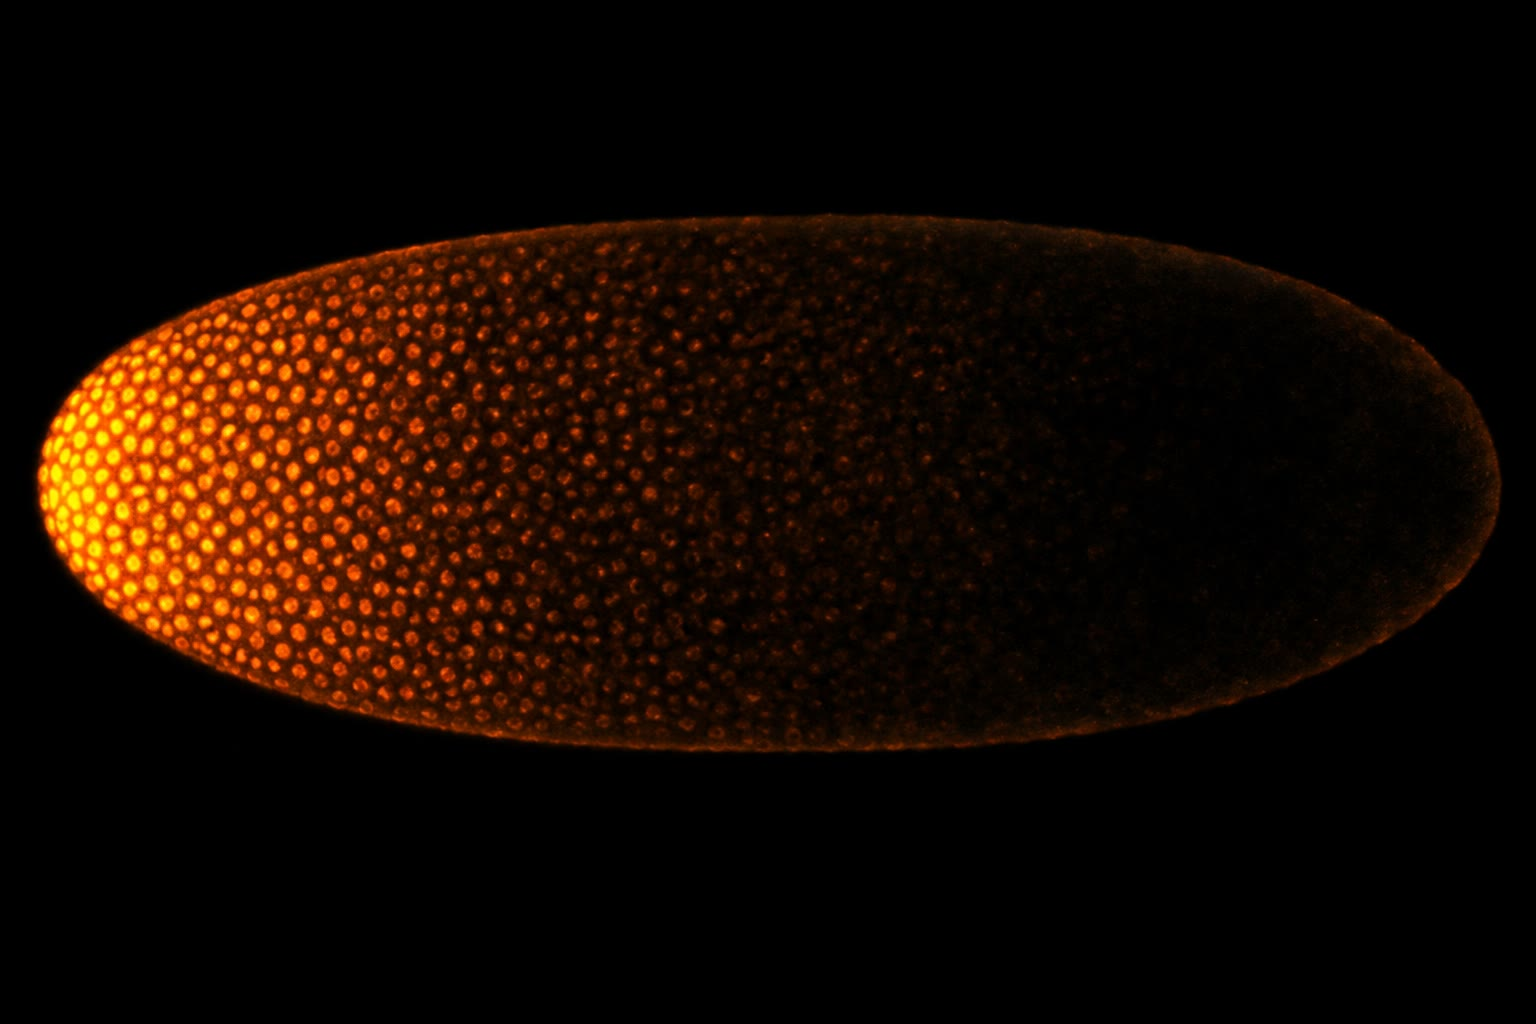
\includegraphics[width=0.46\linewidth]{images/book5/ai/b5-23-bicoid-gradient.jpg}\hspace{0.04\linewidth}
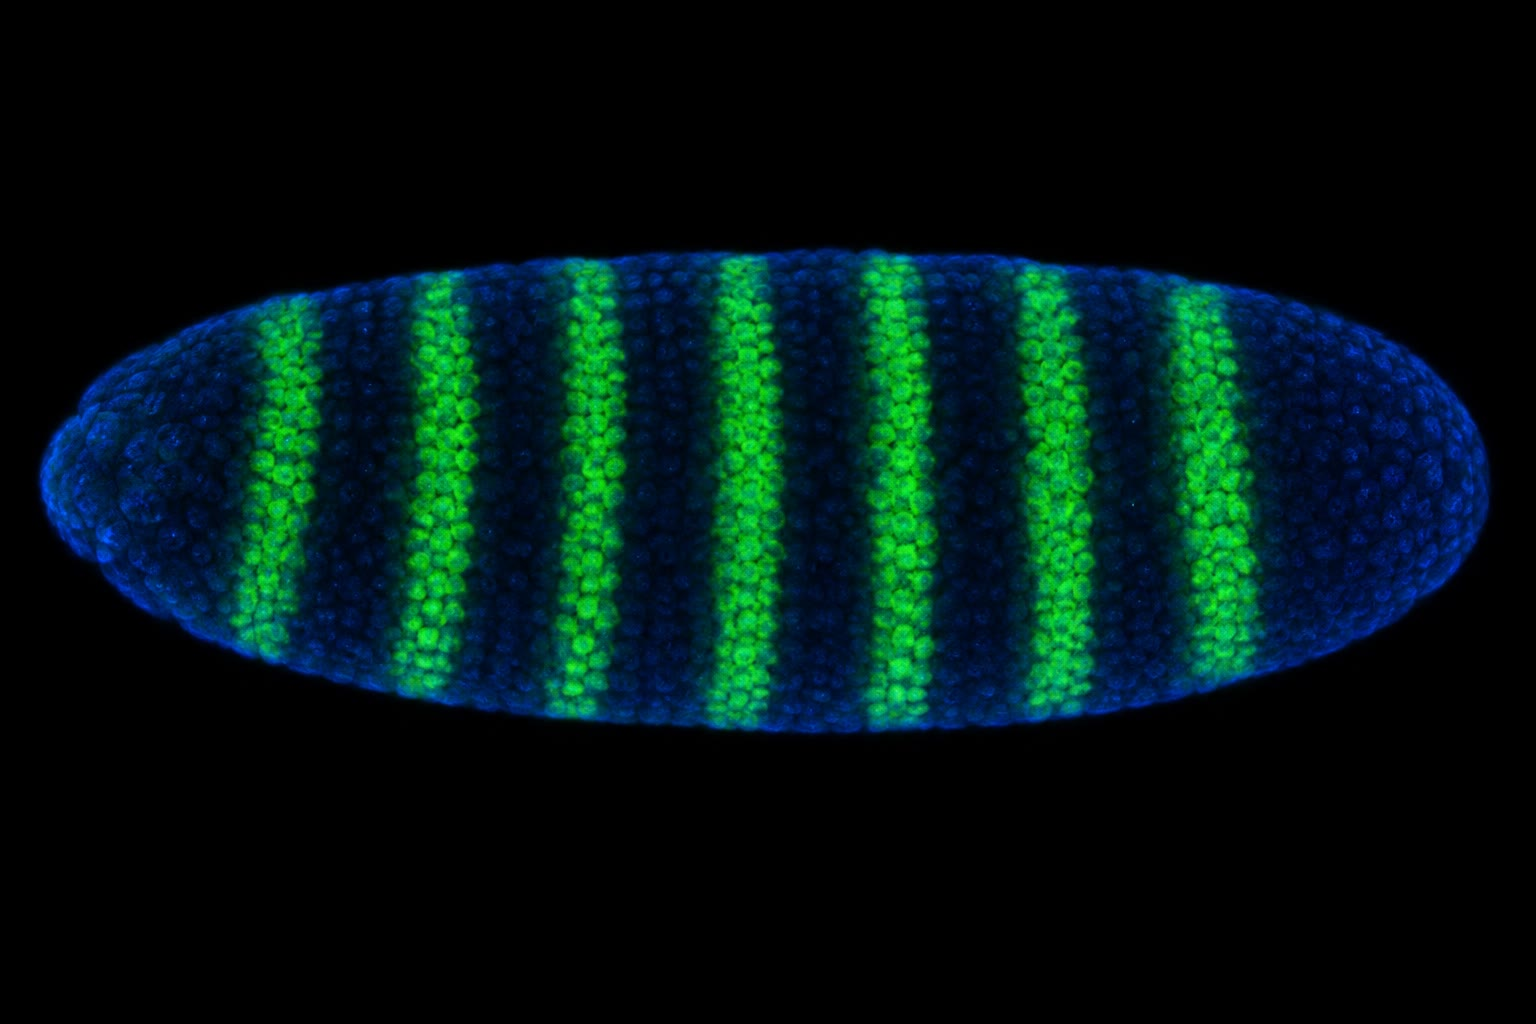
\includegraphics[width=0.46\linewidth]{images/book5/ai/b5-23-embryo-stripes.jpg}

{\small À gauche~: un embryon syncytial marqué pour la protéine Bicoid,
le plus brillant au pôle antérieur et s'estompant exponentiellement vers
le postérieur. À droite~: un embryon, une heure plus tard, marqué pour
une protéine de la règle de parité, sept bandes tracées à partir des
bandes des \omterm{def:b3:developmental-genetics:hierarchy}{gènes gap}.}
\end{omfigure}

\section{L'identité~: les gènes Hox}

\begin{definition}[Gènes homéotiques et colinéarité]\label{def:b3:developmental-genetics:hox}
\index{mutation homéotique}\index{gènes Hox}\index{colinéarité}\index{homéoboîte}\index{code Hox}
Une mutation \emph{homéotique} change une partie du corps en une autre~:
le mot est de Bateson (1894), pour les anomalies qui «~substituent un
membre d'une série à un autre~». Chez la mouche, les mutants dominants
\emph{Antennapedia} font pousser des pattes là où devraient être les
antennes~; les mutants \emph{bithorax} (Lewis, 1978) changent le
troisième segment thoracique en copie du deuxième, de sorte que les
balanciers (haltères) deviennent une seconde paire d'ailes. Les huit
gènes responsables, les \emph{gènes Hox}, sont en deux groupes sur un
même chromosome, et Lewis remarqua que leur ordre le long de l'ADN
correspond à l'ordre le long du corps des segments qu'ils commandent ---
la \emph{colinéarité}, toujours pas pleinement expliquée. Chacun code un
facteur de transcription portant le même domaine de liaison à l'ADN de
60 acides aminés, l'\emph{homéoboîte} (McGinnis, Gehring, 1984), qu'on
trouva ensuite chez tous les animaux~: souris et humains portent quatre
groupes de treize gènes chacun, colinéaires de la même façon, exprimés
en domaines emboîtés le long de l'axe du corps, les gènes les plus
tardifs du groupe étant les plus postérieurs. L'identité d'une cellule
le long de l'axe est donnée par la combinaison des gènes Hox qu'elle
exprime, le \emph{code Hox}~; les gènes postérieurs dominent les
antérieurs (la prévalence postérieure), de sorte que perdre un gène
postérieur laisse le segment prendre l'identité de celui d'avant. Les
gènes Hox ne bâtissent pas un segment~; ils disent à un segment déjà
bâti lequel il est, en allumant les batteries de gènes en aval qui
conviennent à une patte, une aile, une côte ou une vertèbre lombaire.
\end{definition}

\begin{omfigure}
\begin{tikzpicture}[every node/.style={font=\scriptsize}, >=stealth]
  % fly cluster
  \node[left] at (-0.3,2.2) {mouche (\emph{Drosophila}), 8 gènes};
  \foreach \i/\g/\c in {0/lab/omDef, 1/pb/omDef, 2/Dfd/omThm, 3/Scr/omThm, 4/Antp/omMeth, 5/Ubx/omMeth, 6/abd-A/omProp, 7/Abd-B/omProp} {
    \draw[thick, fill=\c!40] ({\i*1.1},1.9) rectangle ({\i*1.1+0.9},2.5); \node[font=\tiny] at ({\i*1.1+0.45},2.2) {\emph{\g}};
  }
  \node[left] at (-0.3,0.9) {groupe HoxB de la souris, 9 sur 13};
  \foreach \i/\g/\c in {0/b1/omDef, 1/b2/omDef, 2/b3/omDef, 3/b4/omThm, 4/b5/omThm, 5/b6/omMeth, 6/b7/omMeth, 7/b8/omProp, 8/b9/omProp} {
    \draw[thick, fill=\c!40] ({\i*1.1},0.6) rectangle ({\i*1.1+0.9},1.2); \node[font=\tiny] at ({\i*1.1+0.45},0.9) {\emph{\g}};
  }
  \draw[->, thick] (0,1.55) -- (9.8,1.55); \node[above, font=\tiny] at (4.9,2.55) {3$'$ $\to$ 5$'$ le long de l'ADN};
  \draw[->, thick] (0,0.2) -- (9.8,0.2); \node[below, font=\tiny] at (4.9,0.05) {antérieur $\to$ postérieur le long du corps};
  % body schematic
  \node[left] at (-0.3,-0.9) {exprimés dans};
  \draw[thick, gray!70, rounded corners=6pt] (0,-1.3) rectangle (9.8,-0.5);
  \foreach \x/\t in {0.6/tête, 2.6/cou, 4.4/thorax, 6.6/lombaire, 8.6/{sacré, queue}} { \node[font=\tiny] at (\x,-0.9) {\t}; }
  \draw[gray!70] (1.6,-1.3) -- (1.6,-0.5); \draw[gray!70] (3.5,-1.3) -- (3.5,-0.5); \draw[gray!70] (5.6,-1.3) -- (5.6,-0.5); \draw[gray!70] (7.6,-1.3) -- (7.6,-0.5);
  \node[below, align=center, font=\tiny] at (4.9,-1.4) {colinéarité~: l'ordre des gènes sur le chromosome est l'ordre de leurs domaines le long du corps~;\\les mêmes groupes, le même ordre, de la mouche à la souris ---\\hérités d'un ancêtre vieux de 600 millions d'années};
\end{tikzpicture}

{\small Les groupes Hox d'une mouche et d'une souris. Les gènes sont
rangés le long de l'ADN dans l'ordre des régions du corps qu'ils
spécifient, chez les deux animaux, et les gènes homologues se
reconnaissent à la séquence~: le gène \emph{Hoxb6} d'une souris est
reconnaissablement l'\emph{Antennapedia} de la mouche.}
\end{omfigure}

\begin{proof}[Faits expérimentaux]
Lewis (1978) cartographia le complexe \emph{bithorax} comme une série de
mutations transformant chacune un segment en celui d'avant, rangées sur
le chromosome dans l'ordre du corps, et proposa que les gènes fussent
activés séquentiellement le long de l'axe. McGinnis et ses collègues
(1984) trouvèrent l'\omterm{def:b3:developmental-genetics:hox}{homéoboîte} par hybridation croisée entre
\emph{Antennapedia} et \emph{Ultrabithorax}, puis chez la grenouille et
la souris. L'équivalence fonctionnelle fut montrée directement~: un gène
\emph{Hoxb6} de souris exprimé chez une mouche produit le phénotype
\emph{Antennapedia}, des pattes à la place des antennes (années 1990)~;
une souris dépourvue de \emph{Hoxc8} a une côte de plus sur sa première
vertèbre lombaire, le segment ayant pris l'identité de celui d'avant~;
et modifier les frontières d'expression des Hox chez le poulet et la
souris déplace l'endroit où se forment les membres antérieurs, la
longueur du cou d'un cygne s'accordant à un recul de la même frontière.
\end{proof}

\begin{omfigure}
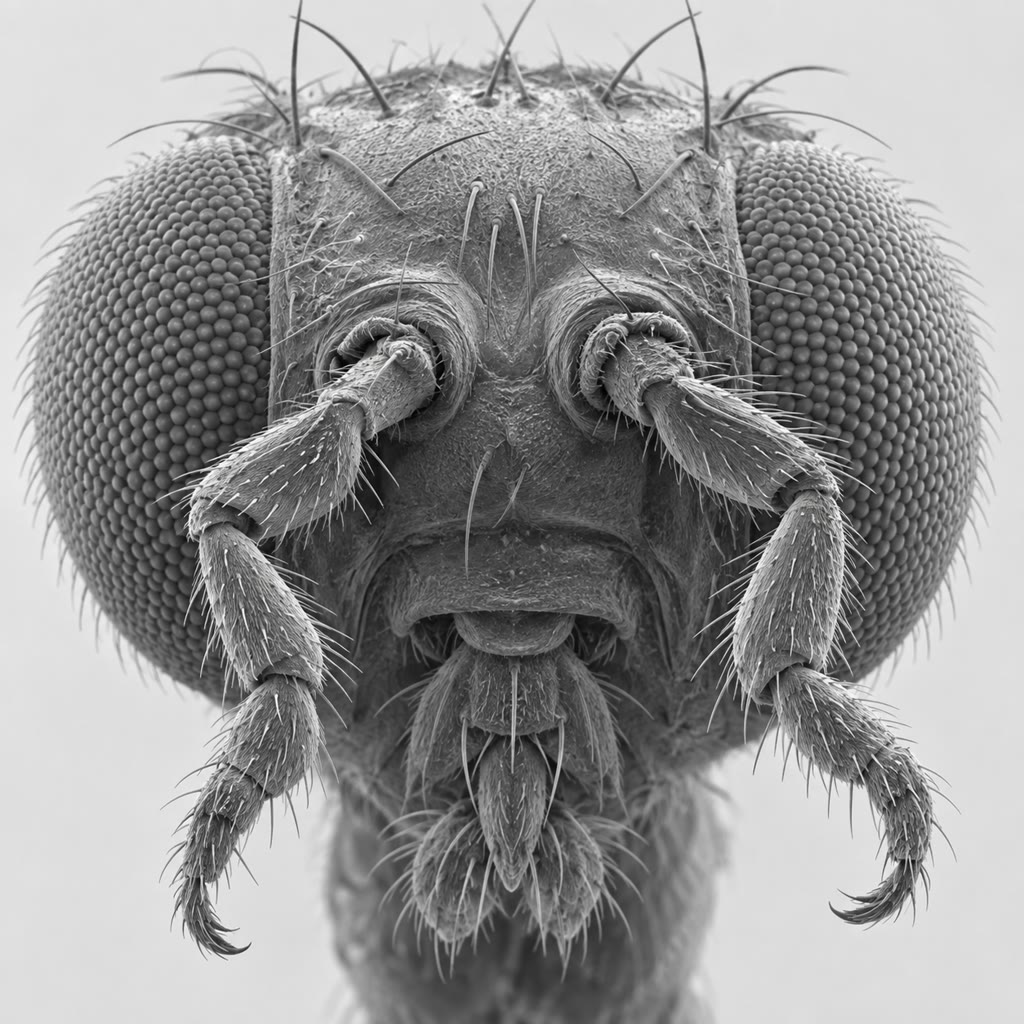
\includegraphics[width=0.34\linewidth]{images/book5/ai/b5-23-antennapedia-fly.jpg}\hspace{0.04\linewidth}
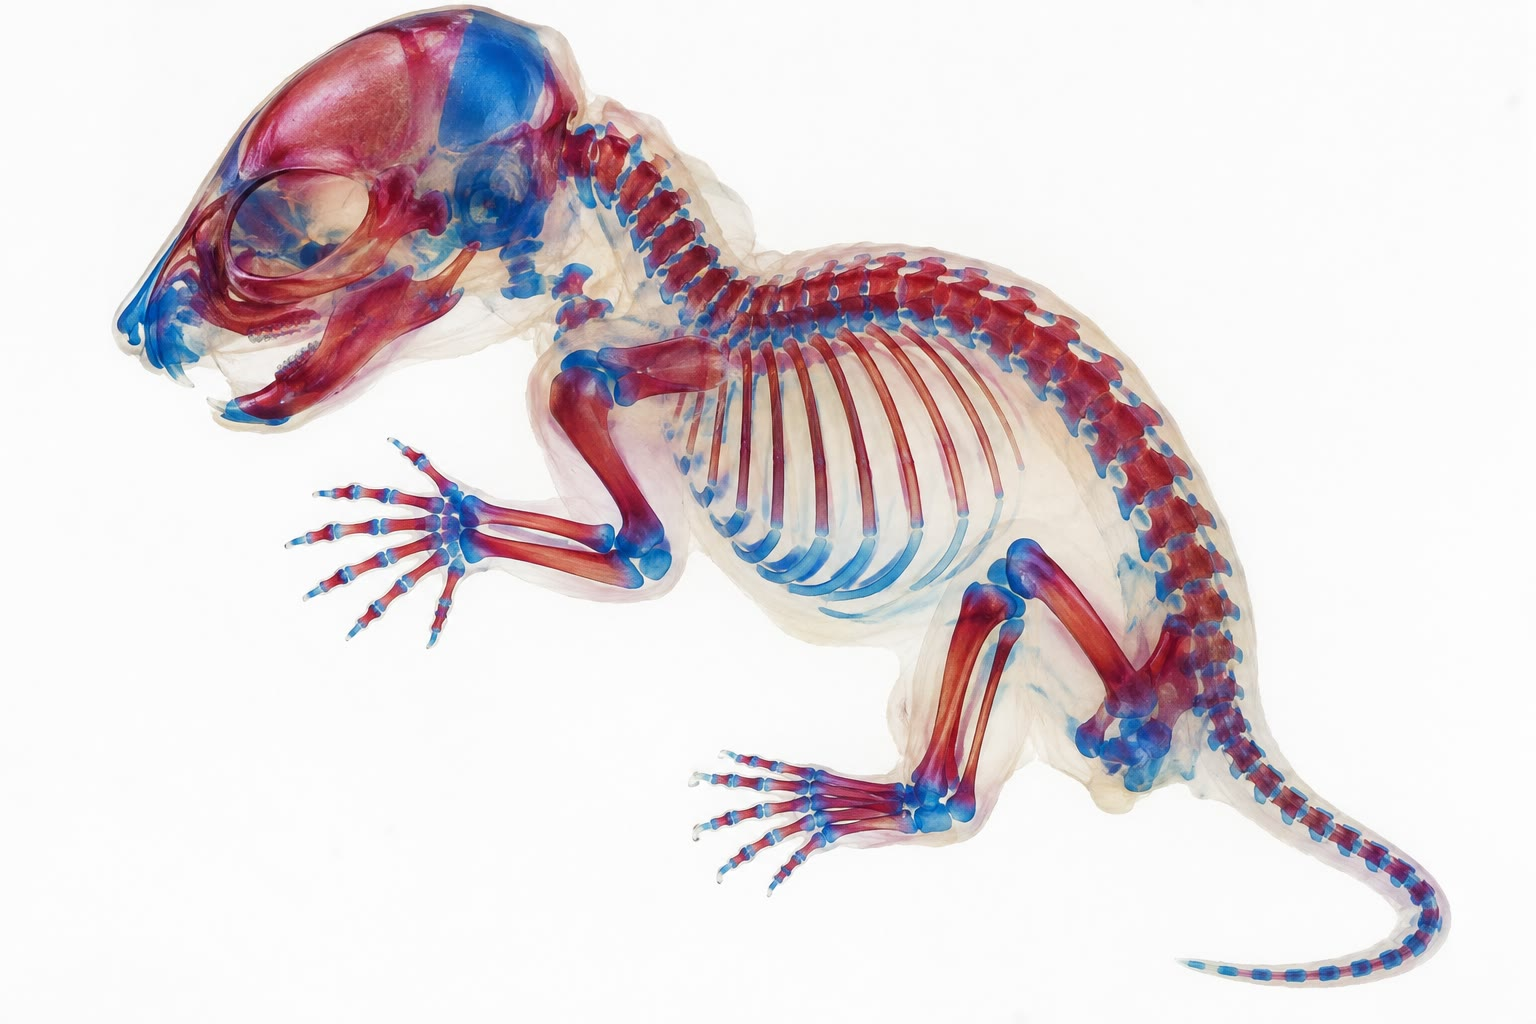
\includegraphics[width=0.5\linewidth]{images/book5/ai/b5-23-limb-skeleton-stain.jpg}

{\small À gauche~: la tête d'une mouche mutante \emph{Antennapedia}, une
paire de pattes là où devraient être les antennes --- le segment bâti
correctement et informé de la mauvaise identité. À droite~: le squelette
d'un embryon de souris, cartilage en bleu et os en rouge, les vertèbres
le long desquelles se lit le \omterm{def:b3:developmental-genetics:hox}{code Hox}.}
\end{omfigure}

\section{Bâtir un vertébré}

\begin{definition}[Organisateurs et centres de signalisation]\label{def:b3:developmental-genetics:organiser}
\index{organisateur}\index{induction}\index{sonic hedgehog}\index{bourgeon de membre}\index{zone d'activité polarisante}\index{crête ectodermique apicale}
Les embryons de vertébrés sont cellulaires dès le départ, de sorte que
leurs gradients sont faits de protéines sécrétées plutôt que de la
diffusion d'un syncytium, et les mêmes quelques familles font tout~:
Wnt, Hedgehog, BMP et d'autres parents du TGF-$\beta$, FGF, Notch et
l'acide rétinoïque. Spemann et Mangold (1924) greffèrent un morceau de
la lèvre dorsale d'une gastrula de triton sur le ventre d'une autre et
obtinrent un second embryon, de la tête à la queue, fait surtout de
cellules de l'hôte~: le greffon était un \emph{organisateur}, qui
induisait ses voisines à former un système nerveux et un axe, et ses
molécules se révélèrent soixante-dix ans plus tard être des antagonistes
sécrétés (Chordine, Noggine) qui bloquent BMP, dont l'absence laisse
l'ectoderme devenir neural --- l'état par défaut. Le \emph{tube neural}
est ensuite structuré du dos au ventre par \emph{sonic hedgehog} venu de
la notochorde et de la plaque du plancher (concentration élevée~:
motoneurones~; basse~: \omterm{def:b3:nervous-systems:cells}{interneurones}) contre BMP venu du toit~; et le
\emph{bourgeon de membre} par deux centres, la \emph{zone d'activité
polarisante} de sa marge postérieure qui sécrète Shh (dont la greffe sur
la marge antérieure donne une duplication en miroir des doigts, six
doigts se rejoignant pouce contre pouce) et la \emph{crête ectodermique
apicale} de sa pointe qui sécrète des FGF qui tiennent en division les
cellules du dessous et spécifient la suite proximale-distale humérus,
avant-bras, main. La greffe, l'ablation et les billes imbibées de
protéine restent les outils~; la logique --- une source locale, un
gradient, des seuils, un code de facteurs de transcription --- est celle
de la mouche.
\end{definition}

\begin{omfigure}
\begin{tikzpicture}[every node/.style={font=\scriptsize}, >=stealth]
  % limb bud
  \fill[omDef!12] (0,0) -- (0,3) .. controls (2.6,3.4) and (3.4,2.2) .. (3.4,1.5) .. controls (3.4,0.8) and (2.6,-0.4) .. (0,0) -- cycle;
  \draw[thick, omDef] (0,0) -- (0,3) .. controls (2.6,3.4) and (3.4,2.2) .. (3.4,1.5) .. controls (3.4,0.8) and (2.6,-0.4) .. (0,0);
  \draw[very thick, omMeth!70!black] (2.9,2.5) .. controls (3.45,1.9) and (3.45,1.1) .. (2.9,0.5);
  \node[right, align=left, omMeth!70!black, font=\tiny] at (3.5,1.5) {crête ectodermique apicale~:\\FGF8~; tient la zone de\\progression en division~;\\proximal $\to$ distal};
  \begin{scope}
    \clip (0,0) -- (0,3) .. controls (2.6,3.4) and (3.4,2.2) .. (3.4,1.5) .. controls (3.4,0.8) and (2.6,-0.4) .. (0,0) -- cycle;
    \foreach \i/\op in {1/50, 2/38, 3/26, 4/14} { \draw[omThm!\op, thick] (0.6,0.5) circle ({0.45*\i}); }
  \end{scope}
  \fill[omThm!50] (0.6,0.5) ellipse (0.5 and 0.35); \node[anchor=north, align=center, omThm, font=\tiny] at (0.9,-0.2) {ZAP~: sonic hedgehog,\\postérieur $\to$ antérieur};
  \node[left, font=\tiny] at (-0.05,2.6) {antérieur}; \node[left, font=\tiny] at (-0.05,0.4) {postérieur};
  \node[left, font=\tiny] at (-0.05,1.5) {paroi du corps};
  \draw[->, thick] (0.3,1.5) -- (3.0,1.5); \node[above, font=\tiny] at (1.75,1.55) {humérus, avant-bras, doigts};
  % right: digit code
  \node[right, align=left] at (7.2,2.6) {identité du doigt selon l'exposition à Shh~:\\pouce (doigt 1)~: aucune~;\\doigts 2 et 3~: le gradient~;\\doigts 4 et 5~: les cellules qui font Shh};
  \node[right, align=left] at (7.2,1.0) {greffer une seconde ZAP en avant~:\\duplication en miroir, 4-3-2-2-3-4~;\\une bille de protéine Shh fait de même};
  \node[right, align=left, gray] at (7.2,-0.2) {la même molécule structure le tube neural\\(motoneurones là où elle est élevée) et l'intestin};
\end{tikzpicture}

{\small Les deux centres de signalisation du \omterm{def:b3:developmental-genetics:organiser}{bourgeon de membre}. Le
\omterm{def:b3:developmental-genetics:organiser}{sonic hedgehog} de la marge postérieure dit aux cellules quel doigt
devenir~; le FGF de la pointe leur dit à quelle distance elles sont le
long du membre. Les greffes qui déplacent un centre déplacent le motif
avec lui.}
\end{omfigure}

\begin{proposition}[Un motif spontané~: le mécanisme de Turing]\label{prop:b3:developmental-genetics:turing}
\index{structure de Turing}\index{réaction--diffusion}\index{activateur--inhibiteur}
Tout motif n'est pas lu dans un gradient préexistant. Turing (1952)
montra que deux substances qui diffusent et réagissent --- un
\emph{activateur} qui stimule sa propre production et celle d'un
\emph{inhibiteur}, et un inhibiteur qui étouffe l'activateur et diffuse
bien plus vite --- peuvent transformer spontanément un champ uniforme en
un réseau régulier de pics~: un petit excès local d'activateur croît par
auto-renforcement tandis que l'inhibiteur qu'il produit se répand et
empêche de nouveaux pics de se former à proximité, de sorte que les pics
apparaissent à un espacement fixé par la portée de l'inhibiteur,
$\lambda \sim \sqrt{D_{\text{inh}}/k_{\text{inh}}}$, et non par une
coordonnée externe. Le mécanisme, dont la partie mathématique est admise
ici, est la meilleure explication des taches et des rayures des pelages,
de l'espacement des follicules pileux et des bourgeons de plumes, des
crêtes du palais, des doigts de la main (dont le nombre monte quand on
raccourcit la longueur d'onde du motif en abaissant l'activité des Hox),
et des rayures du poisson-zèbre, où les cellules qui interagissent ---
des cellules pigmentaires qui repoussent les voisines d'une sorte et
attirent à distance celles d'une autre --- ont été identifiées et leurs
rayures refaites après ablation au laser exactement comme la théorie le
prédit.
\end{proposition}
\admitted

\section{L'évolution des formes}

\begin{definition}[L'évo-dévo]\label{def:b3:developmental-genetics:evodevo}
\index{homologie profonde}\index{boîte à outils génétique}\index{évolution cis-régulatrice}\index{hétérochronie}
Les gènes qui bâtissent les animaux forment une \emph{boîte à outils}
ancienne et partagée~: quelques centaines de facteurs de transcription
et de voies de signalisation présents chez l'ancêtre commun de tous les
animaux, et la diversité animale vient surtout de changements dans
\emph{quand, où et combien} ils sont exprimés plutôt que dans ce qu'ils
codent. L'\emph{homologie profonde}~: le gène \emph{Pax6} dirige la
formation de l'œil chez la mouche, le calmar et la souris, dont les yeux
ne sont pas homologues en tant qu'organes --- un \emph{Pax6} de souris
exprimé sur la patte d'une mouche y fait un œil de mouche ectopique
(Halder, Gehring, 1995). L'\emph{évolution cis-régulatrice}~: la perte
des épines pelviennes chez les épinoches d'eau douce est la délétion
d'un seul activateur du gène \emph{Pitx1}, la protéine restant intacte
et servant toujours ailleurs~; la perte des taches alaires chez
certaines drosophiles, un changement dans un activateur de
\emph{yellow}~; la perte des pattes chez les serpents, un activateur
brisé de \emph{\omterm{def:b3:developmental-genetics:organiser}{sonic hedgehog}} dans le membre. Les \emph{décalages
Hox}~: la frontière d'expression de \emph{Hoxc6} marque la première
vertèbre thoracique chez la souris, le poulet, l'oie et le serpent
pareillement, à la vertèbre 7, 14, 23 et 3~; la perte des pattes
abdominales chez les insectes fut l'acquisition par la protéine Hox Ubx
d'un domaine répresseur qui éteint le gène des pattes
\emph{Distal-less}, là où chez les crustacés il ne le fait pas.
L'\emph{hétérochronie}, un changement dans le tempo d'un programme de
développement, a fait de l'axolotl une larve permanente et du visage
humain celui d'un singe juvénile. La vieille question de l'apparition
des formes nouvelles devient une question d'ADN régulateur~: l'essentiel
du génome qui compte pour la forme n'est pas gène mais interrupteur.
\end{definition}

\begin{example}[Quatre ailes]\label{ex:b3:developmental-genetics:four-wings}
Les ancêtres des mouches avaient quatre ailes, comme en ont encore
libellules et abeilles~; les mouches en ont deux, la paire postérieure
réduite aux balanciers. Chez les mouches, \emph{Ultrabithorax} est
exprimé dans le troisième segment thoracique et y réprime le programme
de l'aile --- une centaine de gènes cibles, un haltère étant une aile
dont ces gènes sont éteints. La mouche triple mutante de Lewis, privée
de la fonction d'\emph{Ubx} dans le troisième segment, fait pousser une
seconde paire d'ailes~: non pas une structure nouvelle, mais la
libération d'une ancienne. Chez les papillons \emph{Ubx} est exprimé
aussi dans l'aile postérieure, et il n'y supprime pas l'aile mais en
change le motif~: la même protéine, un autre jeu de cibles. Quatre cents
millions d'années d'évolution des diptères ont tenu à la décision d'un
seul gène dans un seul segment, et une seule mutation la défait en une
génération --- ce qui explique pourquoi l'histoire des formes se lit
dans les gènes qui les bâtissent.
\end{example}

\begin{remark}[La géométrie tirée de la chimie]\label{rem:b3:developmental-genetics:remark}
Un embryon n'a ni plan ni géomètre. Il a quelques gradients faits de
diffusion et de dégradation, des cellules qui les lisent face à des
seuils et allument des facteurs de transcription, et un code de ces
facteurs qui dit à chaque région ce qu'elle doit devenir~; il a des
\omterm{def:b3:developmental-genetics:organiser}{organisateurs} locaux qui induisent leurs voisines, et des réactions qui
se structurent d'elles-mêmes. La mathématique est celle de la cinétique
du premier ordre et de la diffusion --- une exponentielle, une racine
carrée, un seuil --- et elle explique non seulement où se place la tête
d'une mouche, mais pourquoi doubler un gène décale une frontière d'une
distance fixe, pourquoi six doigts apparaissent quand un signal est
dupliqué, et pourquoi un serpent a trois cents côtes. L'évolution
retouche les interrupteurs, non la machine~: la boîte à outils d'une
éponge et celle d'un humain sont presque la même, et ce qui diffère est
le câblage.
\end{remark}

\section{Exercices}

\begin{exercise}[$\star$]\label{exo:b3:developmental-genetics:1}
Nommer les quatre étages de la hiérarchie de segmentation de la mouche,
un gène de chacun, et le phénotype mutant qui l'a placé dans sa classe.
\end{exercise}

\begin{exercise}[$\star$]\label{exo:b3:developmental-genetics:2}
Qu'est-ce qu'un \omterm{def:b3:developmental-genetics:hierarchy}{gène à effet maternel}~? Une femelle homozygote pour une
mutation nulle de \emph{bicoid} est croisée avec un mâle sauvage~:
décrire ses embryons et expliquer pourquoi leur propre génotype ne les
sauve pas.
\end{exercise}

\begin{exercise}[$\star$]\label{exo:b3:developmental-genetics:3}
Énoncer la \omterm{def:b3:developmental-genetics:hox}{colinéarité} et la prévalence postérieure. Prévoir le
phénotype d'une souris dépourvue de \emph{Hoxc8} et d'une mouche qui
exprime \emph{Antennapedia} dans sa tête.
\end{exercise}

\begin{exercise}[$\star$]\label{exo:b3:developmental-genetics:4}
Qu'a montré la greffe de Spemann et Mangold, et quelles se sont révélées
être les molécules de l'\omterm{def:b3:developmental-genetics:organiser}{organisateur}~? Pourquoi le destin neural
est-il dit «~par défaut~»~?
\end{exercise}

\begin{exercise}[$\star\star$]\label{exo:b3:developmental-genetics:5}
Bicoid~: $D = \qty{4}{\micro m^2/s}$, demi-vie \qty{35}{min}. Calculer
$k$, $\lambda$, et le rapport des concentrations au pôle antérieur et au
milieu de l'œuf (\qty{250}{\micro m}).
\end{exercise}

\begin{exercise}[$\star\star$]\label{exo:b3:developmental-genetics:6}
Avec $\lambda = \qty{100}{\micro m}$, une frontière se place à
\qty{240}{\micro m}. Où se place-t-elle si la mère porte quatre copies
de \emph{bicoid} au lieu de deux~? Une copie~? Exprimer les décalages en
fraction d'un œuf de \qty{500}{\micro m}.
\end{exercise}

\begin{exercise}[$\star\star$]\label{exo:b3:developmental-genetics:7}
Les noyaux du blastoderme sont distants de \qty{8}{\micro m}. Pour
placer une frontière à un noyau près avec $\lambda = \qty{100}{\micro m}$,
avec quelle précision un noyau doit-il lire la concentration de Bicoid~?
Si le noyau compte des molécules pendant un temps $\tau$ et que le
compte suit une loi de Poisson, combien doit-il en compter~?
\end{exercise}

\begin{exercise}[$\star\star$]\label{exo:b3:developmental-genetics:8}
Le gradient approche son état stationnaire à l'échelle de temps $1/k$.
Avec une demi-vie de \qty{35}{min}, quelle fraction de la concentration
stationnaire est atteinte à \qty{60}{min}, \qty{90}{min} et
\qty{120}{min}~? Qu'en déduire pour un embryon qui doit lire le gradient
avant \qty{150}{min}~?
\end{exercise}

\begin{exercise}[$\star\star$]\label{exo:b3:developmental-genetics:9}
Une ZAP est greffée sur la marge antérieure d'un \omterm{def:b3:developmental-genetics:organiser}{bourgeon de membre} de
poulet. Prévoir le motif des doigts, et le motif si l'on y implante à la
place une bille libérant une faible dose de Shh.
\end{exercise}

\begin{exercise}[$\star\star\star$]\label{exo:b3:developmental-genetics:10}
Un morphogène est fabriqué dans tout un tissu de longueur $L$ au débit
$s$ par unité de volume, dégradé au taux $k$, et détruit à la frontière
$x =
L$ (un puits absorbant), sans flux en $x = 0$. Résoudre $Dc'' - kc + s =
0$ pour $c(x)$ et en tracer l'allure. En quoi la forme de ce gradient
diffère-t-elle du cas de la source à une extrémité, et qu'arrive-t-il
quand $L \ll \lambda$~?
\end{exercise}

\begin{exercise}[$\star\star\star$]\label{exo:b3:developmental-genetics:11}
Deux seuils en $T_{1} = 0.3c_{0}$ et $T_{2} = 0.08c_{0}$ divisent un
gradient en trois régions. Montrer que les largeurs des deux premières
régions ne dépendent pas de $c_{0}$, et expliquer pourquoi un embryon
dont la \emph{longueur} varie d'un individu à l'autre (\qty{450}{} à
\qty{550}{\micro m}) a besoin de plus qu'une simple exponentielle pour
mettre son motif à l'échelle. Proposer un mécanisme.
\end{exercise}

\begin{exercise}[$\star\star\star$]\label{exo:b3:developmental-genetics:12}
Les épinoches ont perdu leurs épines pelviennes en supprimant un
activateur de \emph{Pitx1}, les serpents ont perdu leurs membres en
brisant un activateur de \emph{\omterm{def:b3:developmental-genetics:organiser}{sonic hedgehog}}. Expliquer pourquoi les
changements régulateurs plutôt que codants sont la route habituelle vers
une structure perdue ou modifiée, en termes de pléiotropie et de ce que
la même protéine fait ailleurs.
\end{exercise}

\section{Problème~: le drapeau français}

\begin{problem}[{Problème du week-end --- le système de coordonnées d'un
œuf calculé par la cinétique du premier ordre~: la longueur du gradient
de Bicoid, sa source et son temps de formation, les frontières qu'il
trace et leur précision, ce que la dose génique et la taille de l'œuf
leur font, et le code Hox lu en aval, pour finir sur la longueur de
décroissance, le décalage par doublement et la précision de position}]
\label{pb:b3:developmental-genetics:1}
Données~: longueur de l'œuf \qty{500}{\micro m}~; Bicoid $D = \qty{4}{\micro m^2/s}$,
demi-vie \qty{35}{min}~; flux de la source tel que $c_{0} = \qty{50}{nM}$
avec deux copies maternelles~; espacement des noyaux \qty{8.5}{\micro m}
au cycle 14~; seuils $T_{1} = 0.3\,c_{0}$ (tête/thorax) et $T_{2} =
0.08\,c_{0}$ (frontière de \emph{hunchback}) pour le cas à deux copies.
Bruit de lecture $\delta c/c = 0.1$ pour un noyau isolé. Nombre
d'Avogadro \qty{6e23}{}~; un noyau est une sphère de rayon \qty{3}{\micro m}.

\medskip
\noindent\textbf{Partie I --- Le gradient.}
\begin{enumerate}
  \item Calculer $k$ d'après la demi-vie, en \unit{s^{-1}}, et la durée
        de vie $1/k$ en minutes.
  \item Calculer $\lambda = \sqrt{D/k}$ en micromètres. Combien de
        \omterm{thm:b3:developmental-genetics:gradient}{longueurs de décroissance} fait l'œuf~?
  \item De quel facteur la concentration tombe-t-elle d'un pôle à
        l'autre~? De quel facteur sur un espacement nucléaire au milieu
        de l'œuf~?
  \item Calculer le flux de la source $J = c_{0}\sqrt{Dk}$ en
        \unit{nM\,\micro m\,s^{-1}}, et le nombre de molécules qui
        entrent par seconde dans un carré de \qty{1}{\micro m^2} du pôle
        antérieur.
  \item Nombre de molécules de Bicoid dans un noyau au pôle ($c_{0}$) et
        au milieu de l'œuf.
  \item Fraction de l'état stationnaire atteinte à \qty{60}{min} et
        \qty{120}{min} ($1 - \mathrm{e}^{-kt}$). Le gradient est-il
        stationnaire quand les frontières sont tracées, vers
        \qty{120}{min}~?
\end{enumerate}

\medskip
\noindent\textbf{Partie II --- Les frontières.}
\begin{enumerate}[resume]
  \item Positions des deux frontières, en \unit{\micro m} et en fraction
        de la longueur de l'œuf.
  \item La mère a quatre copies~: nouveau $c_{0}$, et les deux positions
        de frontière. De combien chacune s'est-elle déplacée~? Et avec
        six copies~?
  \item Une copie~: positions. Quelles régions ont grandi, lesquelles
        ont rétréci~?
  \item Erreur de position pour un bruit de lecture de \qty{10}{\%}, en
        micromètres et en espacements nucléaires.
  \item Si l'erreur doit valoir un noyau, quelle précision de lecture
        faut-il~? Si le noyau moyenne $n$ lectures indépendantes et que
        le bruit baisse comme $1/\sqrt{n}$, combien de lectures~?
  \item Un noyau situé à la frontière de \emph{hunchback} contient le
        nombre calculé à la question~5. Quel est le bruit de Poisson
        $1/\sqrt{N}$ d'un comptage instantané unique~? Comparer aux
        \qty{10}{\%} et commenter.
\end{enumerate}

\medskip
\noindent\textbf{Partie III --- Mise à l'échelle et robustesse.}
\begin{enumerate}[resume]
  \item Les œufs vont de \qty{450}{} à \qty{550}{\micro m}. Si $\lambda$
        et $c_{0}$ sont fixés, où tombe la frontière de
        \emph{hunchback} en fraction de la longueur de l'œuf dans chaque
        cas~? Le motif est-il mis à l'échelle~?
  \item Supposons plutôt que $D$ varie comme $L^{2}$ (même durée de vie,
        mais une source dont l'étalement croît avec l'œuf). Montrer que
        $\lambda/L$ est alors constant et que le motif est mis à
        l'échelle. Est-ce plausible~?
  \item Le gène \emph{hunchback} répond à Bicoid avec un \omterm{def:b3:structural-biology:allostery}{coefficient de
        Hill} de $5$~: son expression vaut $c^{5}/(c^{5} + T^{5})$. Sur
        combien de micromètres l'expression passe-t-elle de \qty{10}{\%}
        à \qty{90}{\%} autour de la frontière~? Comparer à un espacement
        nucléaire.
  \item Expliquer pourquoi une réponse raide affine une frontière mais
        ne réduit pas à elle seule l'erreur de position due au bruit de
        concentration.
  \item La répression mutuelle entre \omterm{def:b3:developmental-genetics:hierarchy}{gènes gap} affine et stabilise leurs
        frontières. Argumenter en une phrase pourquoi deux gènes qui se
        répriment l'un l'autre ne peuvent être allumés tous deux dans le
        même noyau à l'état stationnaire.
  \item La température élève $D$ de \qty{2}{\%} et $k$ de \qty{6}{\%}
        par degré. Variation de $\lambda$ par degré, et décalage de la
        frontière pour une pièce plus chaude de \qty{5}{\celsius}.
        Pourquoi les embryons auraient-ils besoin d'un mécanisme
        compensateur~?
\end{enumerate}

\medskip
\noindent\textbf{Partie IV --- L'identité.}
\begin{enumerate}[resume]
  \item Le \omterm{def:b3:developmental-genetics:hox}{code Hox}~: avec huit \omterm{def:b3:developmental-genetics:hox}{gènes Hox} de mouche chacun allumé ou
        éteint, combien de codes sont possibles~? Combien sont employés
        (quatorze segments)~? Pourquoi la prévalence postérieure
        réduit-elle le nombre utile~?
  \item Une mouche est privée d'\emph{Ubx} dans son troisième segment
        thoracique. Que devient le segment, et pourquoi le résultat est-il
        quatre ailes et non une structure nouvelle~?
  \item La frontière de \emph{Hoxc6} d'une souris est à la vertèbre 7,
        celle d'une oie à la 23. Que cela prédit-il de leurs cous, et
        qu'est-ce qui a changé au cours de l'évolution~: le gène, ou son
        expression~?
  \item Une greffe de ZAP donne les doigts 4-3-2-2-3-4. Expliquer le
        motif à partir de deux gradients de Shh qui se rencontrent au
        milieu.
  \item Halder et Gehring ont exprimé le \emph{Pax6} de souris dans une
        patte de mouche et y ont obtenu un œil de mouche. Qu'est-ce que
        cela montre du gène, et qu'est-ce que cela ne montre \emph{pas}
        des yeux des mouches et des souris~?
  \item Le sixième doigt~: raccourcir la longueur d'onde de Turing ajoute
        un doigt. Avec cinq doigts en travers d'une plaque de main de
        \qty{2}{mm}, quel changement de longueur d'onde en donne six~?
        Quel paramètre du système de réaction--diffusion le produirait~?
  \item Résumer~: $\lambda$ (question~2), le décalage de frontière par
        doublement de la source (question~8), et l'erreur de position due
        à un bruit de \qty{10}{\%} (question~10).
\end{enumerate}
\end{problem}
